%\section{Event Reconstruction and Analysis} 
For this measurement, the QE-like signal is defined as an event with one muon, no pions and at least one proton with momentum greater than 450 MeV/c exiting the nucleus. A sample of QE-like interactions is selected with at least two reconstructed tracks, one from a muon candidate and at least one proton candidate that stops in the detector. The sample includes both muon tracks that exit the sides of the \minerva detector and those that are matched to a track in the \minos detector. The analysis requires events with a reconstructed interaction vertex in the C, Fe or Pb targets or in the fiducial volume of scintillator.  The event selection uses $\mathrm{d}E/\mathrm{d}x$ to identify protons and to estimate their momentum. The $\mathrm{d}E/\mathrm{d}x$ profile of each hadron is fit to templates for pion and proton hypotheses, and the $\chi^2$ used to determine the particle ID~\cite{Twalton-thesis}.

 Backgrounds from inelastic interactions that produce an untracked pion are reduced by cutting on extra energy $E_{extra}$ that is not linked to a track and is located outside of a 10 cm radius sphere centered at the vertex. The cut on $E_{extra}$ is a function of $Q^2_p$, and is described below. This region around the vertex is excluded to avoid bias due to the mismodeling of low energy nucleons near the vertex~\cite{PhysRevLett.111.022502}. Pions of low kinetic energy are removed by a cut on events with Michel electrons from pion decays near the vertex. A similar event selection criteria have been used in a previous publication for events with interactions in the scintillator \cite{Walton:2014esl}. The present measurement uses the experiment$^{'}$s most current flux prediction~\cite{Aliaga:2013uqz}.

From the measured energy and direction of the proton and muon, the four-momentum transfer \QSqproton and angle between the $\nu$-$\mu$ and $\nu$-p reaction planes, coplanarity angle $\varphi$, are reconstructed.
%To compute the $\QSqproton$ we use the leading proton and assume 
In the case of CCQE scattering from a neutron at rest, \QSqproton can be calculated using the proton kinetic energy, $T_p$ alone.  Under this assumption
%%%%%%%%%%%%%%%%%%%%%%%%%%%%%%%%%%%%%%%%%%%%%%%%%%%%
\begin{equation*}
\QSqproton=(M_{n}-\epsilon_B)^2-M^2_{p}+2(M_{n}-\epsilon_{B})(T_{p}+M_{p}-M_{n}+\epsilon_{B}),
\end{equation*}
%%%%%%%%%%%%%%%%%%%%%%%%%%%%%%%%%%%%%%%%%%%%%%%%%%%%%
where $M_{n,p}$ is the nucleon mass, and $\epsilon_B$ is the effective binding energy of +34 MeV/c$^2$ taken up by liberated nucleons~\cite{Moniz:1971mt}. 

The selected events in the nuclear targets contain two backgrounds, both of which are constrained using data. The first background consists of interactions incorrectly reconstructed in the nuclear targets that originate in the scintillator surrounding the targets.  Figure \ref{targets} shows the simulated scintillator background, as well as the signal from two different nuclear targets (Target 3 and Target 5) as a function of the reconstructed vertex position along the detector longitudinal axis. Scintillator background events are less than $8\%$ of the final sample. 
The level of this background has been constrained by fitting the tails of the vertex distributions in the upstream (US Plastic) and downstream (DS Plastic) regions for each target subsection separately and extracting a scale factor for the scintillator background. Background scale factors span the range from $0.95 \pm 0.05$ (Target 5) to $1.10 \pm 0.05$ (Target 2). The scale factors are applied to the simulated prediction of the scintillator background in the selected sample.
 \begin{figure}[htpb]
\centering
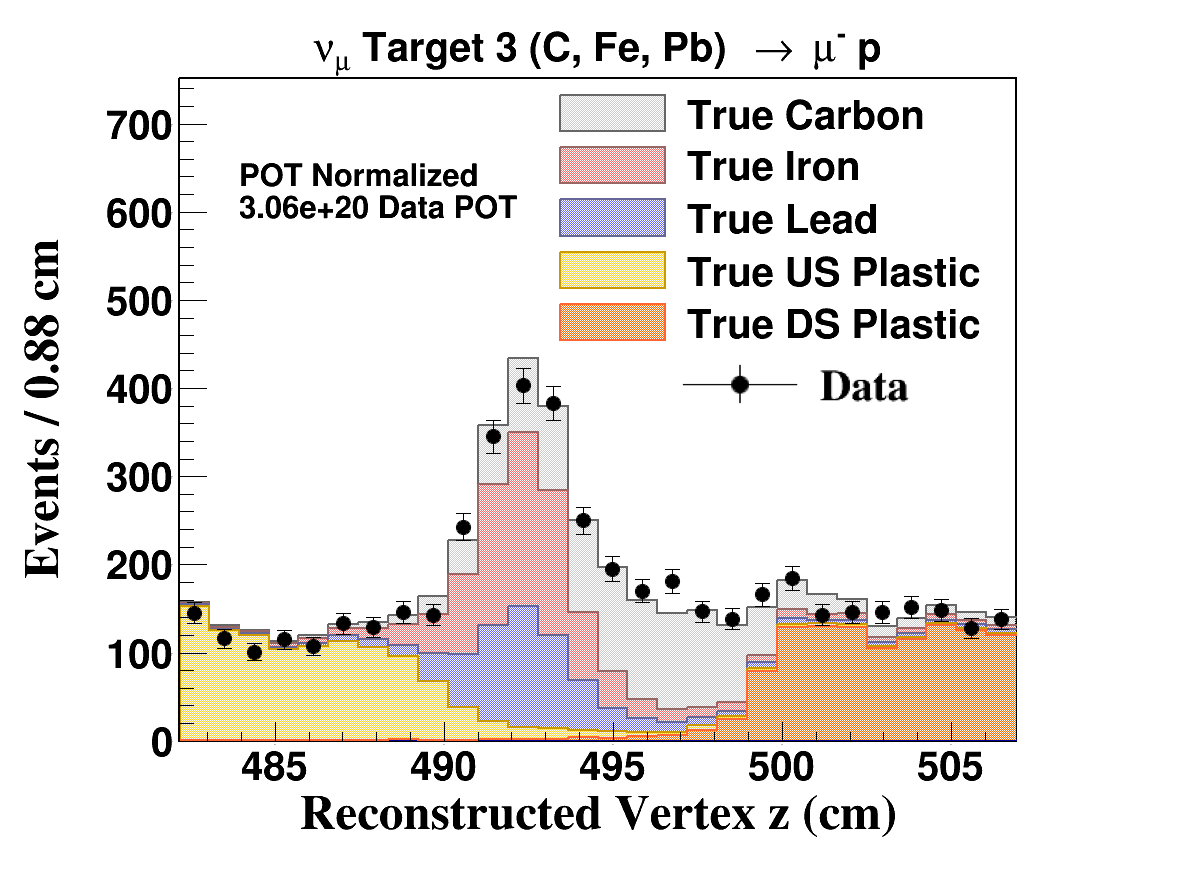
\includegraphics[trim =  0mm 6mm 15mm 2mm, clip, width=0.48\columnwidth]{h_vtx_z_nucleus_genie_var_tar3_data_no_cut_stack2_pot.png}
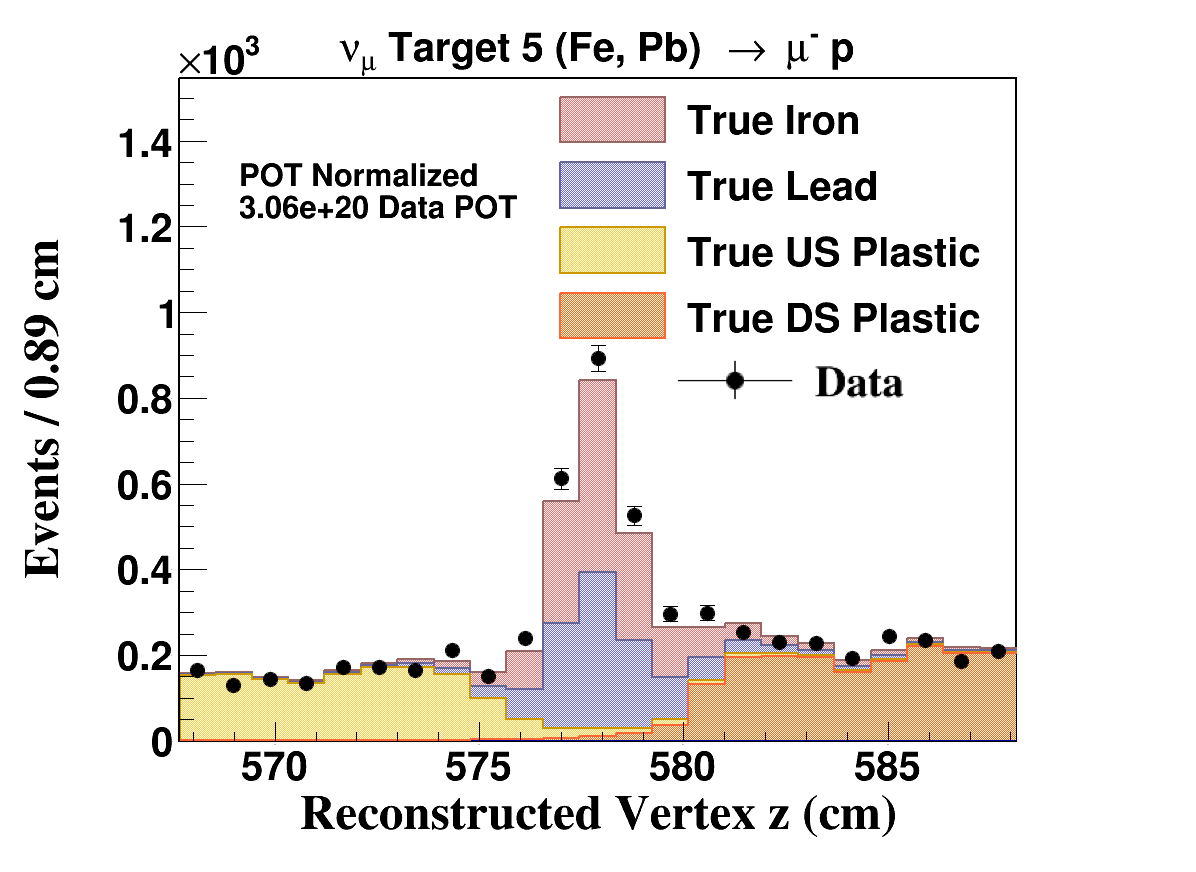
\includegraphics[trim =  0mm 6mm 15mm 2mm, clip, width=0.48\columnwidth]{h_vtx_z_nucleus_genie_var_tar5_data_no_cut_stack4_pot.png}
\caption{Reconstructed interaction vertex $z$ for Target 3 (left) and Target 5 (right). Data and predictions after background tuning are shown for events in each of nucleus. Also shown are contributions from events in the upstream and downstream plastic scintillator.}
\label{targets}
\end{figure}

The second background is from interactions that are not QE-like, mostly baryon resonance production, where the pion is misidentified as a proton. This background is constrained by fitting the distribution of events with $E_{extra}>0.05$ GeV shown in Fig. \ref{sideband}. The fit is performed in bins $\QSqproton<0.5$ GeV$^2$ and $\QSqproton>0.5$ GeV$^2$ of four-momentum transfer for each nucleus (C, Fe and Pb) separately. The fit varies the background normalization while keeping the signal constant, until the simulated distributions match the data distributions. Background scale factors span the range from $(1.01\pm{0.10})$ for C to $(1.3\pm{0.1})$ for Pb. As will be elaborated, pion FSI according to some models introduces a significant $A$-dependence for the QE-like signal, and these same FSI could play a similar role in the background constraint samples.
\begin{figure}[htpb]
\centering
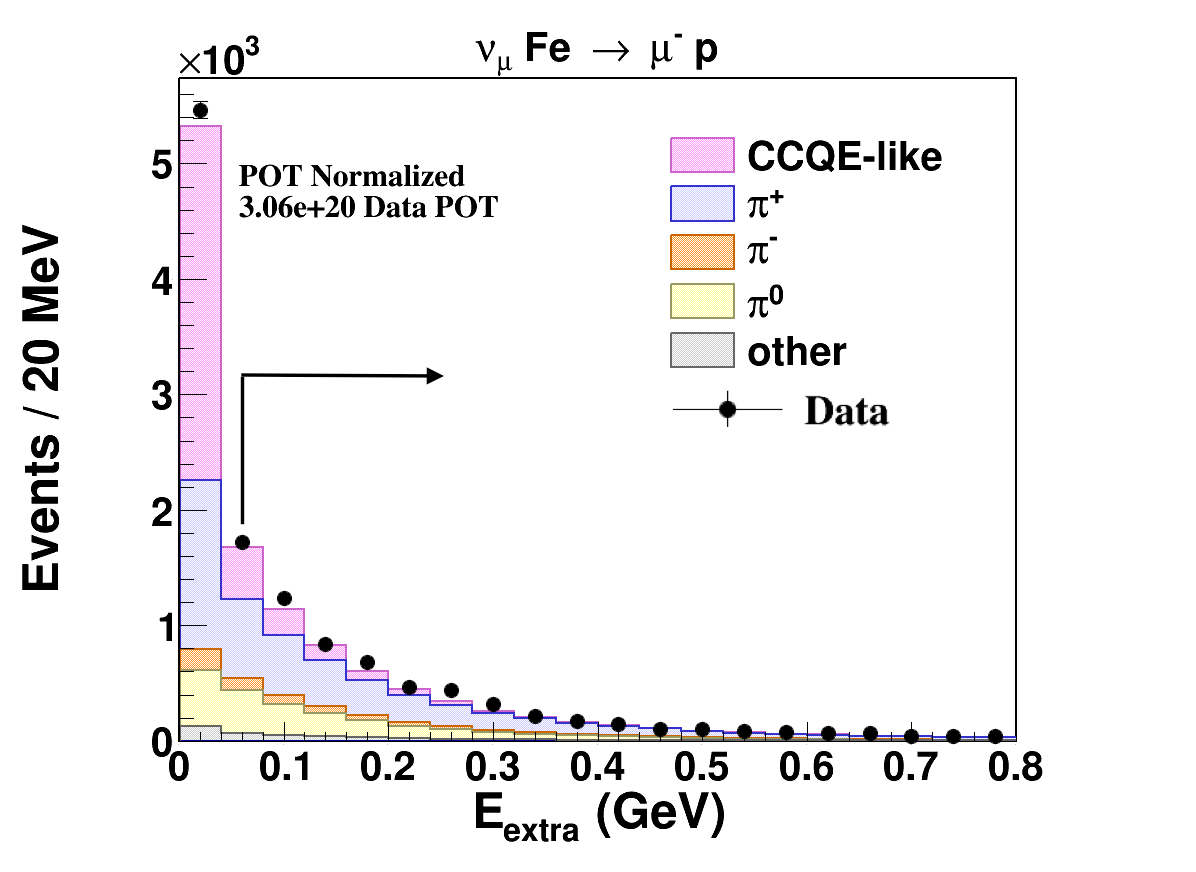
\includegraphics[trim = 0mm 6mm 15mm 2mm, clip, width=0.46\columnwidth]{h_iso_trk_ecal_neutrino_genie_var_nuc26_data_neutrino_ccqe_like_1_pot.png}
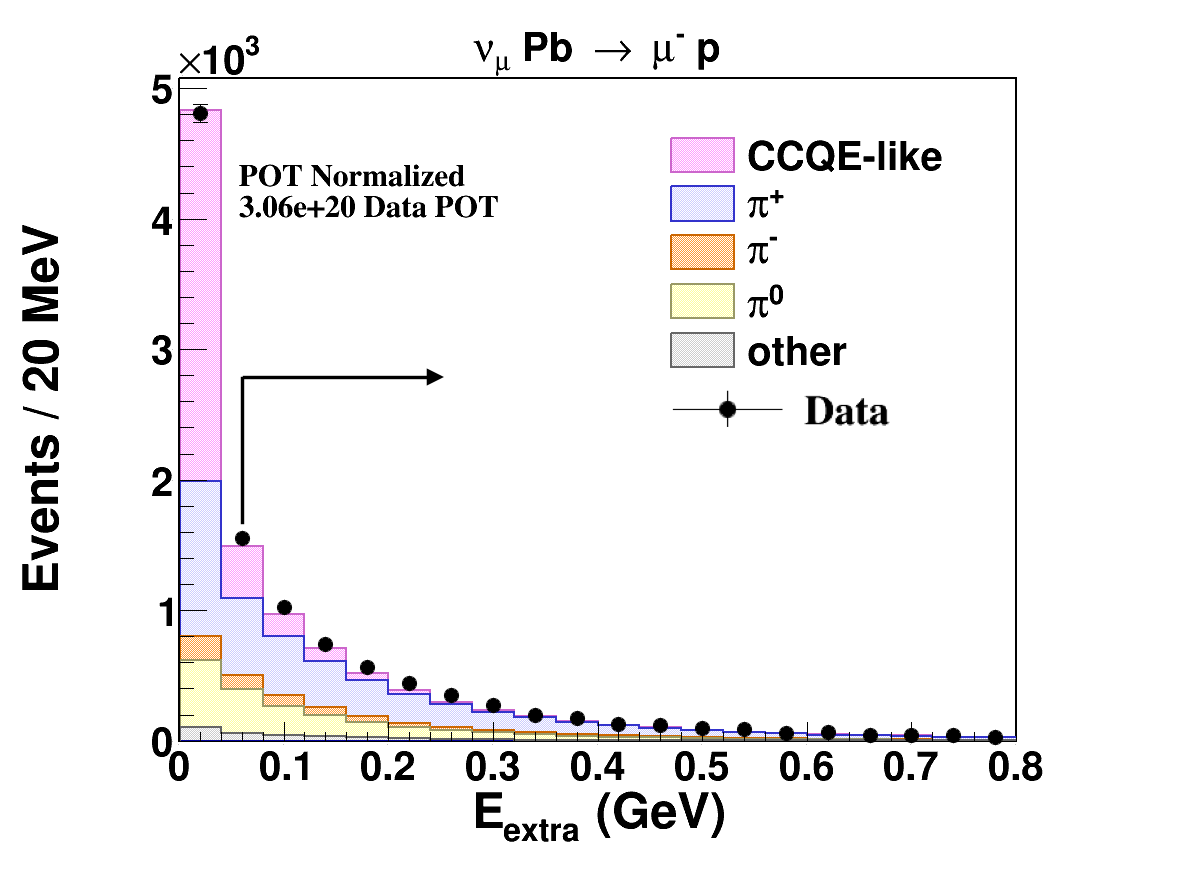
\includegraphics[trim = 0mm 6mm 15mm 2mm, clip, width=0.46\columnwidth]{h_iso_trk_ecal_neutrino_genie_var_nuc82_data_neutrino_ccqe_like_1_pot.png}
\caption{Data and Monte Carlo comparison of the $E_{extra}$ distribution for events in Fe (left) and Pb (right). The MC is after background tuning and is normalized to the same number of protons on target. Predictions for CCQE-like, $\pi^+, \pi^-$ and $\pi^0$ in the final state are shown.   }
\label{sideband}\end{figure}

Separating FSI from initial state nuclear effects is challenging since only the combined effects of both are actually measured.  
The coplanarity $\varphi$, the angle between the $\nu$-$\mu$ and $\nu$-p reaction planes, is sensitive to FSI. For a two-body interaction with a neutron at rest, $\varphi=180^{\circ}$. The detector resolution in $\varphi$ is 3.8$^{\circ}$.  Figure \ref{fig:coplanarity_POT} shows $\varphi$ for events passing the CCQE-like selection for  C (top left), Fe (top right), and Pb (bottom left). The simulation predicts that $30\%$ ($10\%$) of the data is backgrounds from resonance production (deep inelastic scattering); some signal also comes from those processes, plus CCQE-like and 2p2h reactions. The width of the distribution is due to Fermi motion, inelastic scattering, and FSI. FSI broadens the distribution by changing the proton direction and by adding a non-QE component. The distribution without FSI is shown to demonstrate the effect FSI has; the no FSI distribution is too narrow and predicts too few events away from the peak at 180 degrees.  The GENIE FSI model appears to describe the broadening for all three samples, but $A$-dependent discrepancies remain for $\varphi$ near 180 degrees.  
To check the modeling of the $\varphi$ distribution for background events, a set of samples of events with a reconstructed Michel electron has been examined, and good agreement is found in each. One example, for Fe, is shown in the bottom right of Fig.~\ref{fig:coplanarity_POT} with the tuned background scale applied.
\begin{figure}[htpb]
\centering
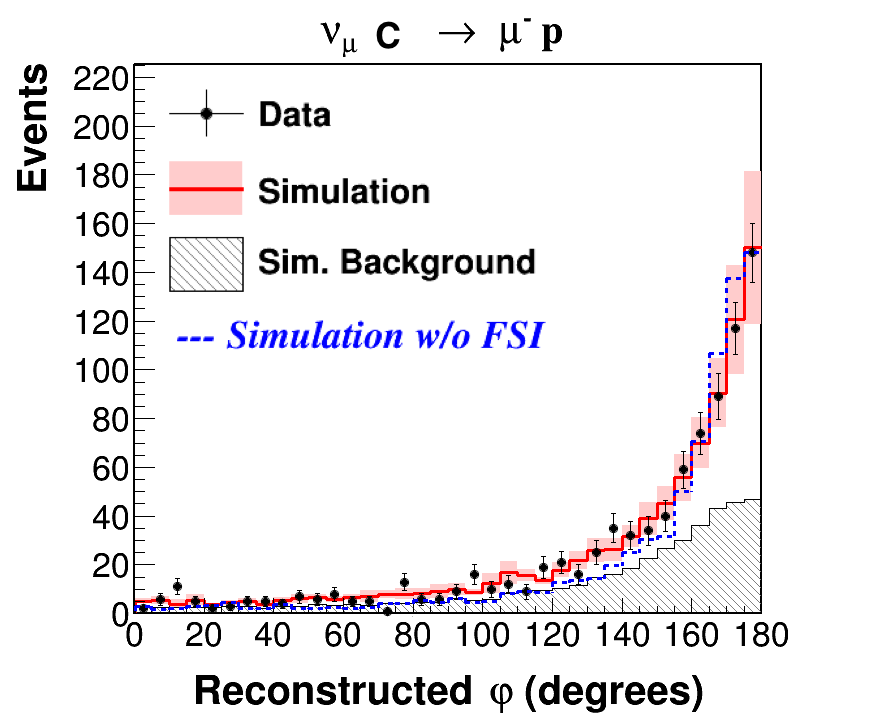
\includegraphics[trim = 0mm 4mm 10mm 2mm, clip, width=0.46\columnwidth]{data-mc_constrained_coplanarity_carbon.png}
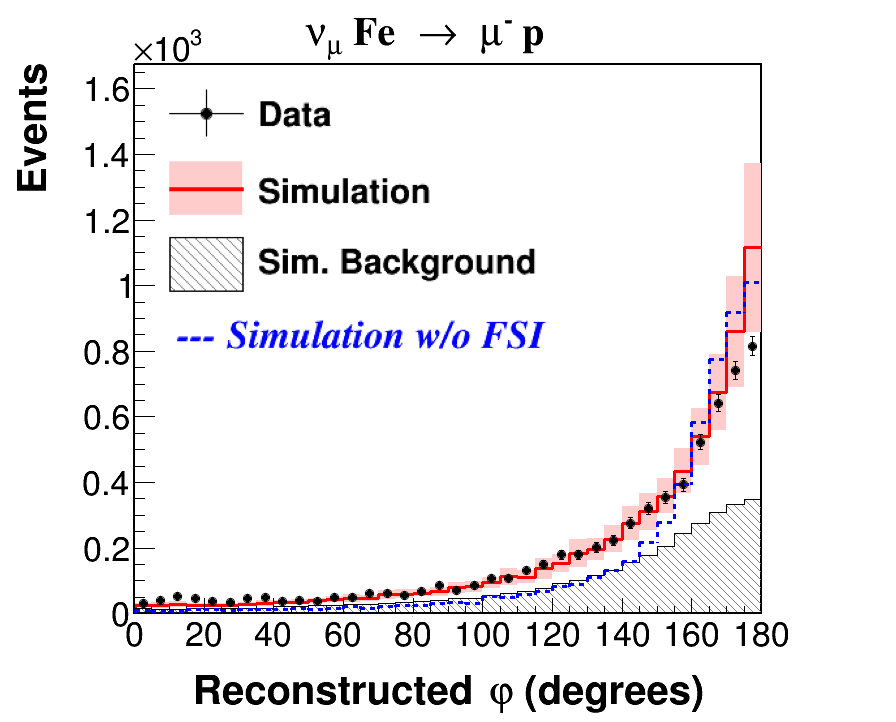
\includegraphics[trim = 0mm 4mm 10mm 2mm, clip, width=0.46\columnwidth]{data-mc_constrained_coplanarity_iron.png}
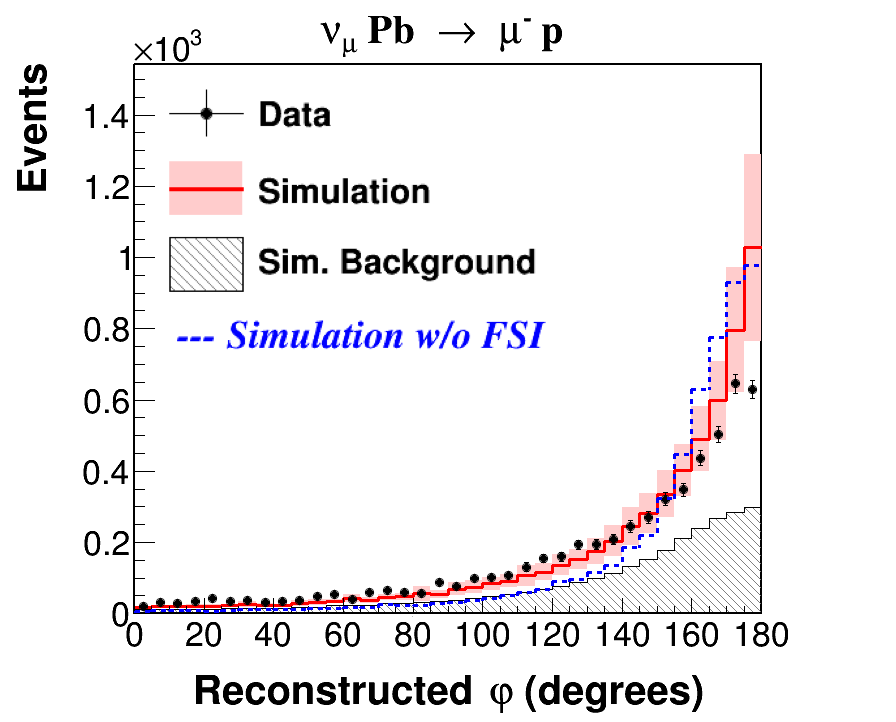
\includegraphics[trim = 0mm 4mm 10mm 2mm, clip, width=0.46\columnwidth]{data-mc_constrained_coplanarity_lead.png}
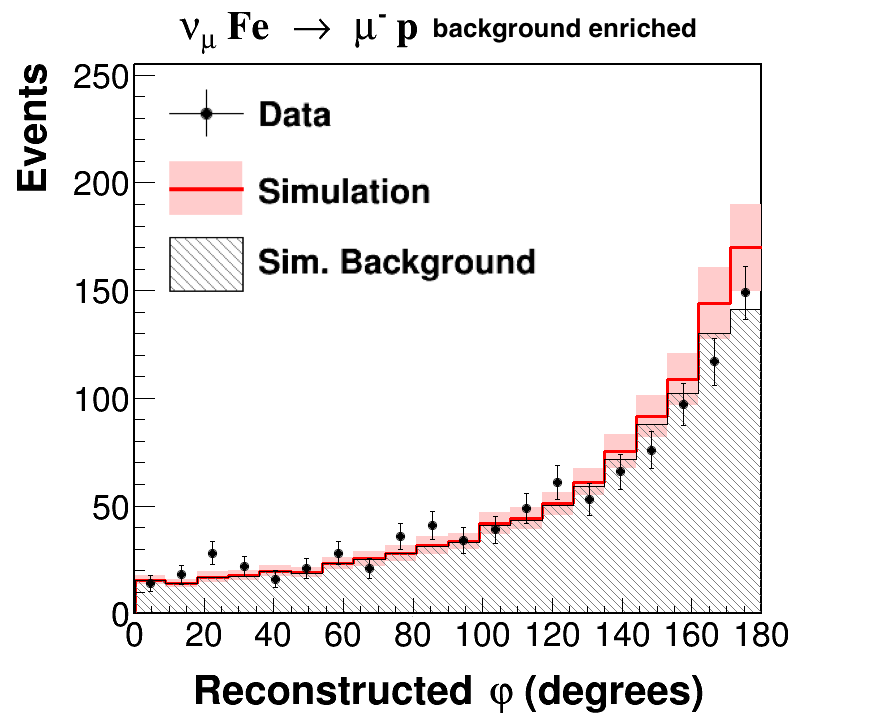
\includegraphics[trim = 0mm 4mm 10mm 2mm, clip, width=0.46\columnwidth]{data-mc_constrained_coplanarity_iron_michel.png}
\caption{ Angle between the neutrino-muon and neutrino-proton planes for the selected events in each nucleus; data and simulation for interactions on carbon (top-left), iron (top-right) and lead (bottom-left). The MC is after background tuning and is normalized to the same number of protons on target. The bottom right plot shows the same distribution in background events, which are dominated by events with a $\pi^+$.}
\label{fig:coplanarity_POT}
\end{figure}

The differential cross section in \QSqproton bin $i$ is calculated using $(\frac{d\sigma}{dQ^2_p})_i=\frac{\sum{U}_{ij}(N_j-B_j)}{\epsilon_i{T}\Phi\Delta(Q^2_p)_i}$, where $N_j$ is the number selected events, $B_j$ is the estimated number of total background events, $\epsilon_i$ is the signal detector efficiency times acceptance, $T$ is the number of target nuclei, $\Phi$ is the integrated neutrino flux, $\Delta(Q^2_p)$ is the width of bin $i$, and $U_{ij}$ is an operation that accounts for the detector smearing of reconstructed \QSqproton. An unfolding method from~\cite{D'Agostini:1994zf} is used; four iterations are performed to obtain the map from reconstructed to true \QSqproton.
